% !TEX encoding = UTF-8 Unicode
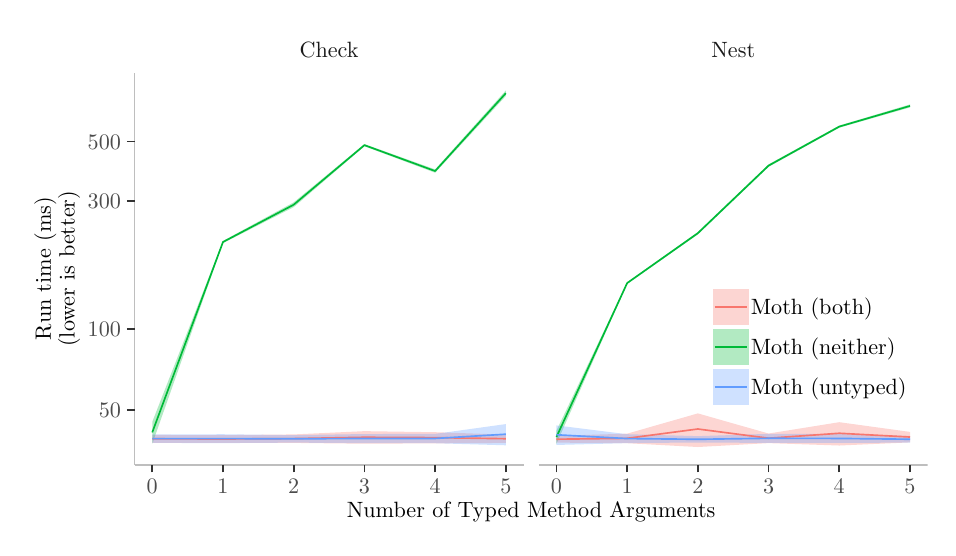
\begin{tikzpicture}[x=1pt,y=1pt]
\definecolor{fillColor}{RGB}{255,255,255}
\path[use as bounding box,fill=fillColor,fill opacity=0.00] (0,0) rectangle (325.21,180.67);
\begin{scope}
\path[clip] ( 38.64, 22.70) rectangle (179.18,164.42);
\definecolor{fillColor}{RGB}{248,118,109}

\path[fill=fillColor,fill opacity=0.30] ( 45.02, 33.50) --
	( 70.58, 33.43) --
	( 96.13, 33.69) --
	(121.68, 34.87) --
	(147.23, 34.49) --
	(172.79, 33.61) --
	(172.79, 30.62) --
	(147.23, 30.47) --
	(121.68, 30.34) --
	( 96.13, 30.62) --
	( 70.58, 30.60) --
	( 45.02, 30.67) --
	cycle;
\definecolor{fillColor}{RGB}{0,186,56}

\path[fill=fillColor,fill opacity=0.30] ( 45.02, 38.22) --
	( 70.58,103.61) --
	( 96.13,117.55) --
	(121.68,138.61) --
	(147.23,129.47) --
	(172.79,157.98) --
	(172.79,156.00) --
	(147.23,128.24) --
	(121.68,137.82) --
	( 96.13,115.82) --
	( 70.58,102.82) --
	( 45.02, 30.28) --
	cycle;
\definecolor{fillColor}{RGB}{97,156,255}

\path[fill=fillColor,fill opacity=0.30] ( 45.02, 33.68) --
	( 70.58, 33.76) --
	( 96.13, 33.43) --
	(121.68, 33.83) --
	(147.23, 33.88) --
	(172.79, 37.43) --
	(172.79, 29.76) --
	(147.23, 30.51) --
	(121.68, 30.54) --
	( 96.13, 30.72) --
	( 70.58, 30.55) --
	( 45.02, 30.62) --
	cycle;
\definecolor{drawColor}{RGB}{248,118,109}

\path[draw=drawColor,line width= 0.6pt,line join=round] ( 45.02, 32.11) --
	( 70.58, 32.04) --
	( 96.13, 32.18) --
	(121.68, 32.66) --
	(147.23, 32.53) --
	(172.79, 32.14);
\definecolor{drawColor}{RGB}{0,186,56}

\path[draw=drawColor,line width= 0.6pt,line join=round] ( 45.02, 34.43) --
	( 70.58,103.22) --
	( 96.13,116.70) --
	(121.68,138.22) --
	(147.23,128.86) --
	(172.79,157.00);
\definecolor{drawColor}{RGB}{97,156,255}

\path[draw=drawColor,line width= 0.6pt,line join=round] ( 45.02, 32.18) --
	( 70.58, 32.18) --
	( 96.13, 32.10) --
	(121.68, 32.22) --
	(147.23, 32.23) --
	(172.79, 33.77);
\end{scope}
\begin{scope}
\path[clip] (184.68, 22.70) rectangle (325.21,164.42);
\definecolor{fillColor}{RGB}{248,118,109}

\path[fill=fillColor,fill opacity=0.30] (191.06, 33.17) --
	(216.62, 33.97) --
	(242.17, 41.29) --
	(267.72, 34.01) --
	(293.27, 38.11) --
	(318.83, 34.60) --
	(318.83, 30.81) --
	(293.27, 29.68) --
	(267.72, 30.55) --
	(242.17, 29.14) --
	(216.62, 30.52) --
	(191.06, 30.72) --
	cycle;
\definecolor{fillColor}{RGB}{0,186,56}

\path[fill=fillColor,fill opacity=0.30] (191.06, 35.05) --
	(216.62, 88.68) --
	(242.17,106.85) --
	(267.72,131.28) --
	(293.27,145.30) --
	(318.83,152.94) --
	(318.83,151.84) --
	(293.27,144.53) --
	(267.72,130.36) --
	(242.17,105.96) --
	(216.62, 88.07) --
	(191.06, 30.30) --
	cycle;
\definecolor{fillColor}{RGB}{97,156,255}

\path[fill=fillColor,fill opacity=0.30] (191.06, 36.95) --
	(216.62, 33.77) --
	(242.17, 33.07) --
	(267.72, 33.89) --
	(293.27, 33.82) --
	(318.83, 33.12) --
	(318.83, 30.74) --
	(293.27, 30.60) --
	(267.72, 30.62) --
	(242.17, 30.77) --
	(216.62, 30.55) --
	(191.06, 29.88) --
	cycle;
\definecolor{drawColor}{RGB}{248,118,109}

\path[draw=drawColor,line width= 0.6pt,line join=round] (191.06, 31.96) --
	(216.62, 32.28) --
	(242.17, 35.65) --
	(267.72, 32.32) --
	(293.27, 34.11) --
	(318.83, 32.75);
\definecolor{drawColor}{RGB}{0,186,56}

\path[draw=drawColor,line width= 0.6pt,line join=round] (191.06, 32.74) --
	(216.62, 88.38) --
	(242.17,106.41) --
	(267.72,130.82) --
	(293.27,144.92) --
	(318.83,152.39);
\definecolor{drawColor}{RGB}{97,156,255}

\path[draw=drawColor,line width= 0.6pt,line join=round] (191.06, 33.56) --
	(216.62, 32.19) --
	(242.17, 31.93) --
	(267.72, 32.29) --
	(293.27, 32.24) --
	(318.83, 31.95);
\end{scope}
\begin{scope}
\path[clip] ( 38.64,164.42) rectangle (179.18,180.67);
\definecolor{drawColor}{gray}{0.10}

\node[text=drawColor,anchor=base,inner sep=0pt, outer sep=0pt, scale=  0.80] at (108.91,169.79) {Check};
\end{scope}
\begin{scope}
\path[clip] (184.68,164.42) rectangle (325.21,180.67);
\definecolor{drawColor}{gray}{0.10}

\node[text=drawColor,anchor=base,inner sep=0pt, outer sep=0pt, scale=  0.80] at (254.95,169.79) {Nest};
\end{scope}
\begin{scope}
\path[clip] (  0.00,  0.00) rectangle (325.21,180.67);
\definecolor{drawColor}{RGB}{190,190,190}

\path[draw=drawColor,line width= 0.6pt,line join=round] ( 38.64, 22.70) --
	(179.18, 22.70);
\end{scope}
\begin{scope}
\path[clip] (  0.00,  0.00) rectangle (325.21,180.67);
\definecolor{drawColor}{gray}{0.20}

\path[draw=drawColor,line width= 0.6pt,line join=round] ( 45.02, 19.95) --
	( 45.02, 22.70);

\path[draw=drawColor,line width= 0.6pt,line join=round] ( 70.58, 19.95) --
	( 70.58, 22.70);

\path[draw=drawColor,line width= 0.6pt,line join=round] ( 96.13, 19.95) --
	( 96.13, 22.70);

\path[draw=drawColor,line width= 0.6pt,line join=round] (121.68, 19.95) --
	(121.68, 22.70);

\path[draw=drawColor,line width= 0.6pt,line join=round] (147.23, 19.95) --
	(147.23, 22.70);

\path[draw=drawColor,line width= 0.6pt,line join=round] (172.79, 19.95) --
	(172.79, 22.70);
\end{scope}
\begin{scope}
\path[clip] (  0.00,  0.00) rectangle (325.21,180.67);
\definecolor{drawColor}{gray}{0.30}

\node[text=drawColor,anchor=base,inner sep=0pt, outer sep=0pt, scale=  0.80] at ( 45.02, 12.24) {0};

\node[text=drawColor,anchor=base,inner sep=0pt, outer sep=0pt, scale=  0.80] at ( 70.58, 12.24) {1};

\node[text=drawColor,anchor=base,inner sep=0pt, outer sep=0pt, scale=  0.80] at ( 96.13, 12.24) {2};

\node[text=drawColor,anchor=base,inner sep=0pt, outer sep=0pt, scale=  0.80] at (121.68, 12.24) {3};

\node[text=drawColor,anchor=base,inner sep=0pt, outer sep=0pt, scale=  0.80] at (147.23, 12.24) {4};

\node[text=drawColor,anchor=base,inner sep=0pt, outer sep=0pt, scale=  0.80] at (172.79, 12.24) {5};
\end{scope}
\begin{scope}
\path[clip] (  0.00,  0.00) rectangle (325.21,180.67);
\definecolor{drawColor}{RGB}{190,190,190}

\path[draw=drawColor,line width= 0.6pt,line join=round] (184.68, 22.70) --
	(325.21, 22.70);
\end{scope}
\begin{scope}
\path[clip] (  0.00,  0.00) rectangle (325.21,180.67);
\definecolor{drawColor}{gray}{0.20}

\path[draw=drawColor,line width= 0.6pt,line join=round] (191.06, 19.95) --
	(191.06, 22.70);

\path[draw=drawColor,line width= 0.6pt,line join=round] (216.62, 19.95) --
	(216.62, 22.70);

\path[draw=drawColor,line width= 0.6pt,line join=round] (242.17, 19.95) --
	(242.17, 22.70);

\path[draw=drawColor,line width= 0.6pt,line join=round] (267.72, 19.95) --
	(267.72, 22.70);

\path[draw=drawColor,line width= 0.6pt,line join=round] (293.27, 19.95) --
	(293.27, 22.70);

\path[draw=drawColor,line width= 0.6pt,line join=round] (318.83, 19.95) --
	(318.83, 22.70);
\end{scope}
\begin{scope}
\path[clip] (  0.00,  0.00) rectangle (325.21,180.67);
\definecolor{drawColor}{gray}{0.30}

\node[text=drawColor,anchor=base,inner sep=0pt, outer sep=0pt, scale=  0.80] at (191.06, 12.24) {0};

\node[text=drawColor,anchor=base,inner sep=0pt, outer sep=0pt, scale=  0.80] at (216.62, 12.24) {1};

\node[text=drawColor,anchor=base,inner sep=0pt, outer sep=0pt, scale=  0.80] at (242.17, 12.24) {2};

\node[text=drawColor,anchor=base,inner sep=0pt, outer sep=0pt, scale=  0.80] at (267.72, 12.24) {3};

\node[text=drawColor,anchor=base,inner sep=0pt, outer sep=0pt, scale=  0.80] at (293.27, 12.24) {4};

\node[text=drawColor,anchor=base,inner sep=0pt, outer sep=0pt, scale=  0.80] at (318.83, 12.24) {5};
\end{scope}
\begin{scope}
\path[clip] (  0.00,  0.00) rectangle (325.21,180.67);
\definecolor{drawColor}{RGB}{190,190,190}

\path[draw=drawColor,line width= 0.6pt,line join=round] ( 38.64, 22.70) --
	( 38.64,164.42);
\end{scope}
\begin{scope}
\path[clip] (  0.00,  0.00) rectangle (325.21,180.67);
\definecolor{drawColor}{gray}{0.30}

\node[text=drawColor,anchor=base east,inner sep=0pt, outer sep=0pt, scale=  0.80] at ( 33.69, 39.72) {50};

\node[text=drawColor,anchor=base east,inner sep=0pt, outer sep=0pt, scale=  0.80] at ( 33.69, 68.94) {100};

\node[text=drawColor,anchor=base east,inner sep=0pt, outer sep=0pt, scale=  0.80] at ( 33.69,115.26) {300};

\node[text=drawColor,anchor=base east,inner sep=0pt, outer sep=0pt, scale=  0.80] at ( 33.69,136.79) {500};
\end{scope}
\begin{scope}
\path[clip] (  0.00,  0.00) rectangle (325.21,180.67);
\definecolor{drawColor}{gray}{0.20}

\path[draw=drawColor,line width= 0.6pt,line join=round] ( 35.89, 42.48) --
	( 38.64, 42.48);

\path[draw=drawColor,line width= 0.6pt,line join=round] ( 35.89, 71.70) --
	( 38.64, 71.70);

\path[draw=drawColor,line width= 0.6pt,line join=round] ( 35.89,118.01) --
	( 38.64,118.01);

\path[draw=drawColor,line width= 0.6pt,line join=round] ( 35.89,139.54) --
	( 38.64,139.54);
\end{scope}
\begin{scope}
\path[clip] (  0.00,  0.00) rectangle (325.21,180.67);
\definecolor{drawColor}{RGB}{0,0,0}

\node[text=drawColor,anchor=base,inner sep=0pt, outer sep=0pt, scale=  0.80] at (181.93,  3.82) {Number of Typed Method Arguments};
\end{scope}
\begin{scope}
\path[clip] (  0.00,  0.00) rectangle (325.21,180.67);
\definecolor{drawColor}{RGB}{0,0,0}

\node[text=drawColor,rotate= 90.00,anchor=base,inner sep=0pt, outer sep=0pt, scale=  0.80] at (  8.36, 93.56) {Run time (ms)};

\node[text=drawColor,rotate= 90.00,anchor=base,inner sep=0pt, outer sep=0pt, scale=  0.80] at ( 17.00, 93.56) {(lower is better)};
\end{scope}
\begin{scope}
\path[clip] (  0.00,  0.00) rectangle (325.21,180.67);
\definecolor{fillColor}{RGB}{255,255,255}

\path[fill=fillColor] (246.90, 72.45) rectangle (261.35, 86.90);
\end{scope}
\begin{scope}
\path[clip] (  0.00,  0.00) rectangle (325.21,180.67);
\definecolor{fillColor}{RGB}{248,118,109}

\path[fill=fillColor,fill opacity=0.30] (247.61, 73.16) rectangle (260.64, 86.19);
\end{scope}
\begin{scope}
\path[clip] (  0.00,  0.00) rectangle (325.21,180.67);
\definecolor{drawColor}{RGB}{248,118,109}

\path[draw=drawColor,line width= 0.6pt,line join=round] (248.34, 79.67) -- (259.91, 79.67);
\end{scope}
\begin{scope}
\path[clip] (  0.00,  0.00) rectangle (325.21,180.67);
\definecolor{fillColor}{RGB}{255,255,255}

\path[fill=fillColor] (246.90, 57.99) rectangle (261.35, 72.45);
\end{scope}
\begin{scope}
\path[clip] (  0.00,  0.00) rectangle (325.21,180.67);
\definecolor{fillColor}{RGB}{0,186,56}

\path[fill=fillColor,fill opacity=0.30] (247.61, 58.70) rectangle (260.64, 71.73);
\end{scope}
\begin{scope}
\path[clip] (  0.00,  0.00) rectangle (325.21,180.67);
\definecolor{drawColor}{RGB}{0,186,56}

\path[draw=drawColor,line width= 0.6pt,line join=round] (248.34, 65.22) -- (259.91, 65.22);
\end{scope}
\begin{scope}
\path[clip] (  0.00,  0.00) rectangle (325.21,180.67);
\definecolor{fillColor}{RGB}{255,255,255}

\path[fill=fillColor] (246.90, 43.54) rectangle (261.35, 57.99);
\end{scope}
\begin{scope}
\path[clip] (  0.00,  0.00) rectangle (325.21,180.67);
\definecolor{fillColor}{RGB}{97,156,255}

\path[fill=fillColor,fill opacity=0.30] (247.61, 44.25) rectangle (260.64, 57.28);
\end{scope}
\begin{scope}
\path[clip] (  0.00,  0.00) rectangle (325.21,180.67);
\definecolor{drawColor}{RGB}{97,156,255}

\path[draw=drawColor,line width= 0.6pt,line join=round] (248.34, 50.76) -- (259.91, 50.76);
\end{scope}
\begin{scope}
\path[clip] (  0.00,  0.00) rectangle (325.21,180.67);
\definecolor{drawColor}{RGB}{0,0,0}

\node[text=drawColor,anchor=base west,inner sep=0pt, outer sep=0pt, scale=  0.80] at (261.35, 76.92) {Moth (both)};
\end{scope}
\begin{scope}
\path[clip] (  0.00,  0.00) rectangle (325.21,180.67);
\definecolor{drawColor}{RGB}{0,0,0}

\node[text=drawColor,anchor=base west,inner sep=0pt, outer sep=0pt, scale=  0.80] at (261.35, 62.46) {Moth (neither)};
\end{scope}
\begin{scope}
\path[clip] (  0.00,  0.00) rectangle (325.21,180.67);
\definecolor{drawColor}{RGB}{0,0,0}

\node[text=drawColor,anchor=base west,inner sep=0pt, outer sep=0pt, scale=  0.80] at (261.35, 48.01) {Moth (untyped)};
\end{scope}
\end{tikzpicture}
